\section{What is a network?}
\begin{itemize}
    \item A network can be defined as a group of computers and other devices connected in some way to be able to exchange data.
        \begin{figure}[H]
            \centering
            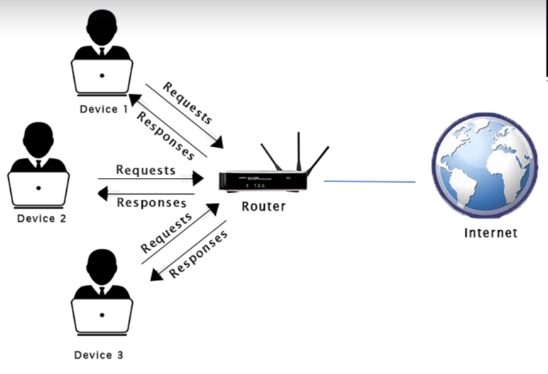
\includegraphics[width=\width\textwidth]{./figs/20230207231418.png}
            %\caption{}
        \end{figure}
\end{itemize}

%%%%%%%%%%%%%%%%%%%%%%%%%%%%%%%%%%%%%%%%%%%%%%%%%%%%%%
\section{Types of networks and its advantages}
\begin{itemize}
    \item There are 2 principle kinds of networks: wide area networks WAN and local area networks LAN.
    \item WAN: 
        \begin{itemize}
            \item Cover cities, countries, and continents.
            \item Based on packet switching technology.
            \item Examples of wan technology: asynchronous transfer mode (ATM), integrated services digital network (ISDN).
        \end{itemize}
    
    \item LAN: 
        \begin{itemize}
            \item Cover buildings or a set of closely related buildings.
            \item Examples of LAN technology: ethernet, token ring, and fibber distributed data interconnect (FDDI).
            \item Ethernet LANs based on a bus topology and bradcast communication.
                \begin{figure}[H]
                    \centering
                    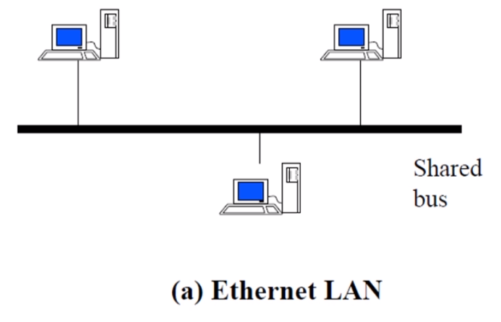
\includegraphics[width=\width\textwidth]{./figs/20230207231750.png}
                    %\caption{}
                \end{figure}
            
            \item Token ring LANs: based on ring topology.
                \begin{figure}[H]
                    \centering
                    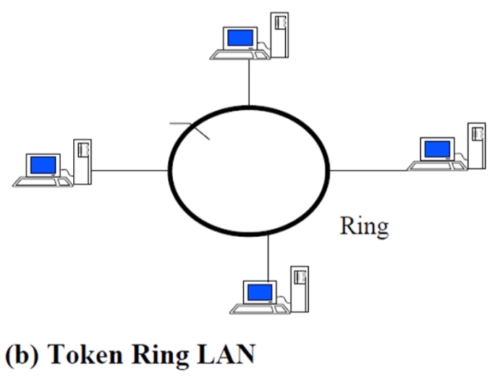
\includegraphics[width=\width\textwidth]{./figs/20230207232047.png}
                    %\caption{}
                \end{figure}
            
            \item FDDI LANs: use optical fibers and an improved token ring mechanism based on two rings flowing in oposite directions.
                \begin{figure}[H]
                    \centering
                    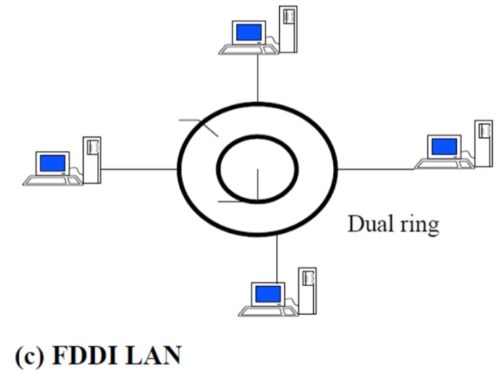
\includegraphics[width=\width\textwidth]{./figs/20230207232146.png}
                    %\caption{}
                \end{figure}
        \end{itemize}
    
    \item Advantages of networks:
        \begin{itemize}
            \item It enhances communication and availability of information.
            \item It allows for more convenient resource sharing.
            \item It makes file sharing easier.
            \item It is highly flexible.
            \item It is an inexpensive system.
            \item It increases cost efficiency.
            \item It boosts storage capacity.
        \end{itemize}
\end{itemize}